\section{优秀的并发-Crossbeam}
默认情况下,Rust标准库的多线程并发是非常安全和方便的,但是,也存在一些特殊情况,
会导致标准库的多线程使用起来受到诸多的限制,比如,在递归函数当中使用多线程:
\begin{code-block}{rust}
use std::thread;
const THRESHOLD: usize = 4;
// 由于Rust的跨线程通信的限制,要求input参数必须是static的生命周期
pub fn find_max(input: &'static [i32]) -> Option<i32> {
    if input.len() <= THRESHOLD {
        return input.iter().cloned().max();
    }
    let middle = input.len() / 2;
    let (left, right) = input.split_at(middle);
    // 由于thread限制,必须使用move关键字
    let thread_left = thread::spawn(move || find_max(left));
    let thread_right = thread::spawn(move || find_max(right));
    let max_left = thread_left.join().unwrap().unwrap();
    let max_right = thread_right.join().unwrap().unwrap();
    Some(max_left.max(max_right))
}
fn main() {
    static ARRAY_REF: &[i32] = &[12, 3, 45, 98, 100, 23, 878, 8765, 123, -897, 866666, 1241];
    let res = find_max(ARRAY_REF);
    info!("The res is {:?}", res);
}
\end{code-block}
由于诸多的限制,上述代码当中,如果需要对多个数组进行排序,则这些数组必须使用static
关键字进行标识,无法处理普通的数组,并且最终会导致生成的二进制文件比较大。

除此之外,比如Rust的通道,只存在多生产者单消费者这一种模式,这也并不符合现实生活
当中的多生产者多消费者的模型。为了改进Rust的并行/并发,目前大多数的开发者使用
Crossbeam\footnote{\url{https://github.com/crossbeam-rs/crossbeam}}替代标准库的thread,
比如,上述的递归函数当中使用多线程,就可以修改为如下的模式:
\begin{code-block}{rust}
extern crate crossbeam;
pub fn find_max_crossbeam(input: &[i32]) -> Option<i32> {
    if input.len() <= THRESHOLD {
        return input.iter().cloned().max();
    }
    let middle = input.len() / 2;
    let (left, right) = input.split_at(middle);
    crossbeam::scope(|s| {
        let thread_left = s.spawn(|_| find_max_crossbeam(left));
        let thread_right = s.spawn(|_| find_max_crossbeam(right));
        let max_left = thread_left.join().unwrap().unwrap();
        let max_right = thread_right.join().unwrap().unwrap();
        Some(max_left.max(max_right))
    })
    .unwrap()
}
fn main() {
    static ARRAY_REF: &[i32] = &[12, 3, 45, 98, 100, 23, 878, 8765, 123, -897, 866666, 1241];
    let res = short_lived::find_max_crossbeam(ARRAY_REF);
    info!("The res is {:?}", res);
    let array = [
        12, 3, 45, 98, 100, 23, 878, 8765, 123, -897, 866666, 12411234,
    ];
    let res = short_lived::find_max_crossbeam(&array);
    info!("The res is {:?}", res);
}
\end{code-block}
通过这样修改的函数,不管是针对static生命周期的还是普通生命周期的数据,都能够自如的处理。

同样的,也可以对Rust标准库的通道(Channel)进行优化,此时,则需要配合使用
\href{https://github.com/crossbeam-rs/crossbeam}{Crossbeam-Channel}。比如下面的例子:
启动2个并行的通道,一个通道负责消息的生产发送,一个通道负责消息的接收和处理:
\begin{code-block}{rust}
use std::thread;
use std::time;

use crossbeam;
use crossbeam_channel;

pub fn channel_usage() {
    let (sender_first, recver_first) = crossbeam_channel::bounded(1);
    let (sender_second, recver_second) = crossbeam_channel::bounded(1);
    let msg_num = 4;
    let worker_number = 8;

    let res = crossbeam::scope(|task| {
        // 生产者
        task.spawn(|_| {
            for i in 0..msg_num {
                if let Ok(_) = sender_first.send(i) {
                    println!("Source send {}", i);
                } else {
                    println!("Faild to send msg from source");
                }
            }
            // 必须手动的将发送端drop
            drop(sender_first);
        });

        // 消费者
        for _ in 0..worker_number {
            let (sender_clone, recver_clone) = (
                sender_second.clone(), recver_first.clone());
            task.spawn(move |_| {
                thread::sleep(time::Duration::from_millis(50));
                for msg in recver_clone.iter() {
                    println!("Worker {:?} received {}",
                        thread::current().id(), msg);
                    if let Err(err) = sender_clone.send(msg * 2) {
                        println!("Failed to send complete message: {:?}", err);
                    }
                }
            });
        }

        // 同样,必须要将发送端drop
        drop(sender_second);

        for msg in recver_second.iter() {
            println!("The result is {}", msg);
        }
    });

    if let Ok(_) = res {}
}
\end{code-block}

在上述的代码当中,使用的是\codeinline{rust}{bounded}这种有缓冲的通道。这里的通道的
概念,和Rust当中本身的通道概念,以及Tokio当中的通道概念是相同的。同理,也可以crossbeam
也提供了无缓冲的通道:
\begin{code-block}{rust}
pub fn unbounded_channel() {
    let (sender, recevier) = crossbeam_channel::unbounded();
    let msg_number = 5;
    if let Ok(_) = crossbeam::scope(|task| {
        task.spawn(|_| {
            for i in 0..msg_number {
                if let Ok(_) = sender.send(i) {
                    thread::sleep(time::Duration::from_millis(100));
                }
            }
        });
    }) {
        for _ in 0..msg_number {
            if let Ok(msg) = recevier.recv() {
                println!("Received message :{}", msg);
            }
        }
    }
    drop(sender);
}
\end{code-block}

\begin{note}
虽然在上述代码当中,我们使用的是\codeinline{rust}{crossbeam_channel},但是
实际上它是\codeinline{rust}{crossbeam}的一部分,因此,实际使用当中,我们也可以使用
\codeinline{rust}{crossbeam::channel}来替代它。不仅仅是channel,crossbeam当中的很多模块都
被拆分成为了的独立的crate,可以单独使用。具体的对应关系可参考下表\colorunderlineref{table:crossbeam_crate}:
\begin{table}[H]
  \caption{crossbeam拆分的crate}
  \label{table:crossbeam_crate}
  \rowcolors{2}{gray!80!}{black!50!white}
  \begin{tabularx}{\textwidth}{
  |m{\dimexpr.50\linewidth-2\tabcolsep-1.3333\arrayrulewidth}% column 1
  |m{\dimexpr.50\linewidth-2\tabcolsep-1.3333\arrayrulewidth}% column 2
  |}
  \hline
  \centering origin path & \centering\arraybackslash crate\\ \hline
  \codeinline{rust}{crossbeam::channel} & \codeinline{rust}{crossbeam_channel} \\
  \codeinline{rust}{crossbeam::deque} & \codeinline{rust}{crossbeam_deque} \\
  \codeinline{rust}{crossbeam::epoch} & \codeinline{rust}{crossbeam_epoch} \\
  \codeinline{rust}{crossbeam::queue} & \codeinline{rust}{crossbeam_queue} \\
  \codeinline{rust}{crossbeam::utils} & \codeinline{rust}{crossbeam_utils} 包含:
  \begin{itemize}
      \item atomic
      \item sync
      \item thread
  \end{itemize}
  \\ \hline
  \end{tabularx}
\end{table}
\end{note}

不过,Crossbeam能够提供的功能和特性,远远不止上述的内容。

\subsection{线程安全的Cell}
Rust本身提供了一个\codeinline{rust}{Cell/RefCell}用于处理内部的可变性,但是,这
2个类型并不是线程安全的,也就是说,只能在单线程环境当中使用。而Crossbeam则提供了
线程安全的Cell:\codeinline{rust}{AtomicCell}。该类型和标准库当中的\codeinline{rust}{Cell}
的使用非常类似,但还有一些其他的用法:
\begin{code-block}{rust}
use crossbeam::atomic;

fn test_crossbeam_atomic_cell() {
    let instance = atomic::AtomicCell::new(21);

    // 获取cell当中的值
    let load_value = instance.load();
    assert_eq!(21, load_value);

    // 写入cell当中的值
    instance.store(128);
    assert_eq!(128, instance.load());

    // 与特定的值进行交换
    instance.swap(256);
    assert_eq!(256, instance.load());

    // 将cell当中的元素取出,cell当中替换为类型的默认值
    let take_value = instance.take();
    assert_eq!(0, instance.load());
    assert_eq!(256, take_value);

    // 将cell与0进行比较,如果相等,则将cell当中的值替换为100
    let res = instance.compare_exchange(0, 100);
    // 成功,则会返回Ok(cell的原始值)
    assert_eq!(res, Ok(0));
    let res = instance.compare_exchange(0, 200);
    // 失败,则返回Err(cell的原始值)
    assert_eq!(res, Err(100));

    let res = instance.compare_exchange(instance.load(), 300);
    assert_eq!(300, instance.load());
    assert_eq!(res, Ok(100));

    // 取出cell当中的值,并将cell消费掉
    let instance_value = instance.into_inner();
    // 后续无法在使用instance变量,该变量的生命周期已经结束
    assert_eq!(21, instance_value);
}
\end{code-block}

由于\codeinline{rust}{AtomicCell}的线程安全性,因此,可以直接在多线程当中进行使用:
\begin{code-block}{rust}
pub fn unbounded_channel() -> u32 {
    use crossbeam::atomic;
    // 需要指定cell的类型,便于后面的计算
    let instance = atomic::AtomicCell::<u32>::new(21);
    let (sender, recevier) = crossbeam_channel::unbounded();
    let msg_number = 5;
    if let Ok(_) = crossbeam::scope(|task| {
        task.spawn(|_| {
            for i in 0..msg_number {
                if let Ok(_) = sender.send(i) {
                    instance.fetch_add(i);
                    thread::sleep(time::Duration::from_millis(100));
                }
            }
        });
    }) {
        for _ in 0..msg_number {
            if let Ok(msg) = recevier.recv() {
                println!("Received message :{}", msg);
            }
        }
    }

    drop(sender);
    instance.into_inner()
}
\end{code-block}

在上述的代码当中,并没有看到常用的锁机制,这涉及到一个问题:哪些数据类型在被\codeinline{rust}{AtomicCell}
包裹之后,不需要使用锁,即\colorblock{无锁操作的}:
\begin{code-block}{rust}
fn test_crossbeam_atomic_lock() {
    assert_eq!(true, atomic::AtomicCell::<usize>::is_lock_free());
    assert_eq!(atomic::AtomicCell::<()>::is_lock_free(), true);
    struct Foo {
        bar: isize,
    }
    assert_eq!(atomic::AtomicCell::<Foo>::is_lock_free(), true);
    struct FooComplexe {
        bar: isize,
        status: bool,
    }
    assert_eq!(atomic::AtomicCell::<FooComplexe>::is_lock_free(), false);
    assert_eq!(atomic::AtomicCell::<[u8; 10]>::is_lock_free(), false);
}
\end{code-block}
也即是说,常见的普通类型基本都是无锁的,包含单个字段,且字段类型为基本类型的结构体
也是无锁的,但是多个字段的结构体就不是无锁了,同理,数组和切片,也都不是无锁类型。
无锁的数据类型,在操作时通常会使用原子锁;而有锁的数据类型,则只能使用全局锁,只是这个
全局锁的处理是由Crossbeam以及Rust来处理的,针对用户则是透明的,使用起来与无锁数据类型
的区别不大:
\begin{code-block}{rust}
pub fn unbounded_channel_lock() {
    use crossbeam::atomic;
    let array: [u8; 5] = [1, 2, 3, 4, 5];
    let instance = atomic::AtomicCell::new(array);
    let (sender, recevier) = crossbeam_channel::unbounded();
    let msg_number = 5;
    if let Ok(_) = crossbeam::scope(|task| {
        task.spawn(|_| {
            for i in 0..msg_number {
                if let Ok(_) = sender.send(i) {
                    let mut instance_value = instance.load();
                    instance_value[i] = instance_value[i] + 10 as u8;
                    instance.store(instance_value);
                    thread::sleep(time::Duration::from_millis(100));
                }
            }
        });
    }) {
        for _ in 0..msg_number {
            if let Ok(msg) = recevier.recv() {
                println!("Received message :{}", msg);
            }
        }
    }

    println!("{:?}", instance.load());

    drop(sender);
}
\end{code-block}

\subsection{channel}
如同上述代码所示,crossbeam也提供了通道的功能,不过,不同的是,crossbeam只提供了
2种类型的通道:
\begin{itemize}
  \item \codeinline{rust}{bounded} 即容量有限的通道
  \item \codeinline{rust}{unbounded} 即容量没有限制的通道
\end{itemize}

通常情况下,通道的用法和其他crate当中的类似,但是,针对\codeinline{rust}{bounded}
类型的通道,有一个比较特殊的例子,即容量为0的通道。这种类型的通道无法容纳任何信息,
发送和接收需要同时出现,以便配对的进行消息传递:
\begin{code-block}{rust}
fn test_channel_bounded_zero_capacity() {
    let (non_sender, non_recevier) = crossbeam_channel::bounded(0);
    thread::spawn(move || {
        non_sender.send("hello world").unwrap();
        drop(non_sender);
    });

    assert_eq!(Ok("hello world"), non_recevier.recv());
    drop(non_recevier);

    let (non_sender, non_recevier) = crossbeam_channel::bounded(0);
    thread::spawn(move || {
        assert_eq!(non_recevier.recv(), Ok("hello world"));
        drop(non_recevier);
    });

    non_sender.send("hello world").unwrap();
    drop(non_sender);
}
\end{code-block}

与此同时,crossbeam还支持共享通道,发送者1的消息,接收者2可以处理,同理,接收者1
可以处理发送者2的消息:
\begin{code-block}{rust}
fn test_crossbeam_shared_channel() {
    let (first_sender, first_recevier) = crossbeam_channel::bounded(0);
    let (second_sender, second_recevier) = (first_sender.clone(), first_recevier.clone());

    thread::spawn(move || {
        assert_eq!(second_recevier.recv(), Ok("This is the first sender"));
        second_sender.send("This is the second sender").unwrap();
    });

    first_sender.send("This is the first sender").unwrap();
    assert_eq!(first_recevier.recv(), Ok("This is the second sender"));
}
\end{code-block}
注意,clone操作只会为相同的发送端或接收端创建一个新的句柄,\colorblock{不会以任何方式创建单独的消息流},
即消息在所有的发送端/接收端都是共享的。
\begin{code-block}{rust}
let (sender_1, recevier_1) = crossbeam_channel::unbounded();
let (sender_2, recevier_2) = (sender_1.clone(), recevier_1.clone());
let (sender_3, recevier_3) = (sender_1.clone(), recevier_1.clone());
thread::spawn(move || {
    sender_1.send(10).unwrap();
    sender_2.send(20).unwrap();
    sender_3.send(30).unwrap();
});

// 任何一个接收端都可以接收消息,但是,接收之后,
// 消息就从队列当中消失了。
assert_eq!(recevier_3.recv(), Ok(10));
assert_eq!(recevier_1.recv(), Ok(20));
assert_eq!(recevier_2.recv(), Ok(30));
\end{code-block}

非常特别的是,接收端和发送端还可以通过引用进行共享,这是其他的框架(tokio,std)所
不具备的能力:
\begin{code-block}{rust}
let (scope_sender, scope_receiver) = crossbeam_channel::bounded(0);
crossbeam::thread::scope(|task| {
    task.spawn(|_| {
        let recv = scope_receiver.recv().unwrap();
        println!("task received {}", recv);
        scope_sender.send(100).unwrap();
    });
    scope_sender.send(200).unwrap();
    let recv = scope_receiver.recv().unwrap();
    assert_eq!(100, recv);
})
.unwrap();
drop(scope_sender);
assert_eq!(true, scope_receiver.is_empty());
\end{code-block}

Crossbeam的通道同样可以作为迭代器进行使用:
\begin{code-block}{rust}
fn test_crossbeam_channel_iter() {
    let (sender, receiver) = crossbeam_channel::unbounded();
    thread::spawn(move || {
        sender.send(1).unwrap();
        sender.send(2).unwrap();
        sender.send(3).unwrap();
        drop(sender);
    });

    // 以迭代器的方式使用通道
    /*
    let v: Vec<_> = receiver.iter().collect();
    println!("result is {:?}", v);
    */
    for item in receiver {
        println!("result is {:?}", item);
    }
}
\end{code-block}

如果存在多个通道,但是只需要其中任意一个通道的结果,则可以使用\codeinline{rust}{select!}
宏。这个宏的定义,与tokio的类似:
\begin{code-block}{rust}
fn test_crossbeam_channel_select() {
    let (sender_first, recevier_first) = crossbeam_channel::unbounded();
    let (sender_second, recevier_second) = crossbeam_channel::unbounded();
    thread::spawn(move || {
        sender_first.send(10).unwrap();
    });
    thread::spawn(move || {
        sender_second.send(100).unwrap();
    });

    // 下面2种是相同的
    // crossbeam_channel::select! {
    crossbeam::channel::select! {
        recv(recevier_first) -> message_first => println!(
            "The first message is {:?}", message_first),
        recv(recevier_second) -> message_second=> println!(
            "The second message is {:?}", message_second),
        default(std::time::Duration::from_secs(10)) => println!("timeout"),
    }
}
\end{code-block}
Crossbeam的\codeinline{rust}{select!}宏是对\codeinline{rust}{Select}结构体的一个
简单的二次封装,在上述代码当中的\codeinline{rust}{recv}以及\codeinline{rust}{default}
等函数,实际上是\codeinline{rust}{Select}结构体的一些方法。关于\codeinline{rust}{select!}
及其本质的介绍,将在后面进行展开,此处不再进行。

在crossbeam当中,还有一类比较特殊的通道:时间通道。时间通道主要包含了3大类型:
\begin{itemize}
  \item{item} after:在具体时间之后传递单条消息的通道
  \item{item} tick:如字面意思,定期传送单条消息的通道
  \item{item} never:永远不会发送消息的通道
\end{itemize}

其中,after和tick通道比较常用:
\begin{code-block}{rust}
fn test_crossbeam_time_channel() {
    let start = time::Instant::now();
    let ticker = crossbeam_channel::tick(time::Duration::from_millis(50));
    let after__ = crossbeam_channel::after(time::Duration::from_secs(5));

    loop {
        crossbeam_channel::select! {
            // 接收定时通道的消息
            recv(ticker) -> _ => println!("Now elapsed :{:?}", start.elapsed()),
            // 接收after通道的消息
            recv(after__) -> _ => {
                println!("Now is time out");
                break;
            },
        }
    }
}
\end{code-block}

而never通道比较特殊,经常用于错误处理的场合(比如放在unwrap当中):
\begin{code-block}{rust}
fn test_crossbeam_never_channel() {
    let (sender, recevier) = crossbeam_channel::unbounded();
    thread::spawn(move || {
        thread::sleep(time::Duration::from_secs(1));
        sender.send(100).unwrap();
    });

    let duration = Some(time::Duration::from_millis(50));
    let timeout = duration
        // 通过after通道发送信息
        .map(|d| crossbeam_channel::after(d))
        // 如果发送失败,则使用never通道,即永远也不发送
        .unwrap_or(crossbeam_channel::never());

    crossbeam_channel::select! {
        recv(recevier) -> msg => println!("The result is {:?}", msg),
        recv(timeout) -> _ => println!("Time out"),
    }
}
\end{code-block}

除上述三种时间通道之外,还有一种比较特殊的时间通道:at,用于指定在特定的时间执行
特定的动作:
\begin{code-block}{rust}
fn test_crossbeam_at_channel() {
    let (sender, recevier) = crossbeam_channel::unbounded();

    // 从当前时间开始5秒之后
    let do_action = time::Instant::now() + time::Duration::from_secs(5);
    thread::spawn(move || {
        thread::sleep(time::Duration::from_secs(10));
        sender.send(100).unwrap();
    });

    crossbeam_channel::select! {
        // 接收特定时间段的通道消息
        recv(crossbeam_channel::at(do_action)) -> _ => println!("time out"),
        recv(recevier) -> msg => println!("The message is {:?}", msg),
    }
}
\end{code-block}

\subsection{select宏与Select结构体}
Crossbeam的通道有多种使用方式,同样的,\codeinline{rust}{select!}宏也有多种应用方式。
在实际的使用当中,\codeinline{rust}{select!}宏的使用方式大致如下:
\begin{code-block}{rust}
crossbeam_channel::select! {
    // 从接收端接收通道的消息
    recv(recevier) -> msg => do_something,
    // 作为发送端,send的第二个参数为向通道当中发送的消息
    send(sender, 20) -> res => do_something,
    // 默认操作,即无法满足之前的所有分支条件
    default => do_something
}
\end{code-block}

上述伪代码当中,\codeinline{rust}{recv}和\codeinline{rust}{send}都是\codeinline{rust}{Select}
结构体的方法。同样的,\codeinline{rust}{default}同样是结构体的方法,但是,该方法
或者说该分支比较特殊,可以如同上面一样,只是作为标识符使用,也可以当作函数使用,
可以接收参数:
\begin{code-block}{rust}
select! {
    recv(r1) -> msg => panic!(),
    recv(r2) -> msg => panic!(),
    default(Duration::from_millis(100)) => println!("timed out"),
}
\end{code-block}

不管\codeinline{rust}{select!}宏的使用方法如何变化,其本质上,还是对\codeinline{rust}{Select}结构体
的一种封装。该结构体允许定义一组通道操作,等待其中任何一个操作准备就绪,并最终执行它;
如果多个操作同时准备好,则随机选择其中的一个。与该结构体相比,\codeinline{rust}{select!}
宏无法动态的创建通道列表。\codeinline{rust}{Select}结构体的使用大致如下:
\begin{code-block}{rust}
fn test_crossbeam_select_struct() {
    let (sender, receiver) = crossbeam_channel::unbounded::<u8>();
    let mut sel = crossbeam_channel::Select::new();
    let idx = sel.send(&sender);
    // 完成select操作
    let oper = sel.select();
    // 利用操作者完成真正的业务
    oper.send(&sender, 12).unwrap();

    let idx_r = sel.recv(&receiver);
    let oper = sel.select();
    let res = oper.recv(&receiver).unwrap();

    println!("The idx is {}, {}, ={}", idx, idx_r, res);
}
\end{code-block}

但是很明显,上述的代码并没有如同\codeinline{rust}{select!}宏一般的优雅便于使用,
而事实上,上述代码也只是对宏的一种拙劣模仿,真正的实现则如同下面代码所示:
\begin{code-block}{rust}
fn test_crossbeam_select_implement() {
    let (sender, receiver) = crossbeam_channel::unbounded();
    let (sender_2, receiver_2) = crossbeam_channel::unbounded();

    thread::spawn(move || {
        thread::sleep(time::Duration::from_secs(1));
        sender.send(10).unwrap();
    });

    thread::spawn(move || {
        sender_2.send(20).unwrap();
    });

    let mut sel = crossbeam_channel::Select::new();

    // 创建2个操作通道分支
    let operator1 = sel.recv(&receiver);
    let operator2 = sel.recv(&receiver_2);

    // 启动select操作
    let operation = sel.select();

    // 等待通道返回结果
    match operation.index() {
        // 根据通道索引进行对应的操作
        idx if idx == operator2 => println!(
            "The recevier second  received {:?}",
            operation.recv(&receiver_2)
        ),
        idx if idx == operator1 => {
            println!("The recevier received {:?}", operation.recv(&receiver))
        }
        _ => unreachable!(),
    }
}
\end{code-block}

如果select操作的时间太长,还可以如同宏一样,添加超时等待机制:
\begin{code-block}{rust}
...
// 设定select的操作时间为500ms
let oper = sel.select_timeout(Duration::from_millis(500));
match oper {
    // select操作超时
    Err(_) => panic!("should not have timed out"),
    Ok(oper) => match oper.index() {
        i if i == oper1 => assert_eq!(oper.recv(&r1), Ok(10)),
        i if i == oper2 => assert_eq!(oper.recv(&r2), Ok(20)),
        _ => unreachable!(),
    }
}
...
\end{code-block}

当然,还可以要求select操作在指定时间之前完成,否则也当作超时处理:
\begin{code-block}{rust}
...
// 设置具体的时间点,表示从现在开始后的500ms
let deadline = Instant::now() + Duration::from_millis(500);
// 设置select的超时时间
let oper = sel.select_deadline(deadline);
match oper {
    // select操作超时
    Err(_) => panic!("should not have timed out"),
    // select操作正常完成
    Ok(oper) => match oper.index() {
        i if i == oper1 => assert_eq!(oper.recv(&r1), Ok(10)),
        i if i == oper2 => assert_eq!(oper.recv(&r2), Ok(20)),
        _ => unreachable!(),
    }
}
...
\end{code-block}

在实际的操作当中,除了使用\codeinline{rust}{Select}结构体的\codeinline{rust}{select}
函数之外,同样可以使用\codeinline{rust}{ready}系列函数。比如上述的示例代码,可以通过
该系列函数进行改写:
\begin{code-block}{rust}

// 通常的用法,阻塞模式
...
let mut sel = crossbeam_channel::Select::new();
let operator1 = sel.recv(&receiver);
let operator2 = sel.recv(&receiver_2);

match sel.ready() {
    idx if idx == operator1 => assert_eq!(receiver.recv(), Ok(10)),
    idx if idx == operator2 => assert_eq!(receiver_2.try_recv(), Ok(20)),
    _ => unreachable!(),
}
...

// 通常的用法,非阻塞模式
...
match sel.try_ready() {
    Err(_) => panic!("both operations should be ready"),
    Ok(i) if i == oper1 => assert_eq!(r1.try_recv(), Ok(10)),
    Ok(i) if i == oper2 => assert_eq!(r2.try_recv(), Ok(20)),
    Ok(_) => unreachable!(),
}
...

// 超时设置
...
match sel.ready_timeout(Duration::from_millis(500)) {
    Err(_) => panic!("should not have timed out"),
    Ok(i) if i == oper1 => assert_eq!(r1.try_recv(), Ok(10)),
    Ok(i) if i == oper2 => assert_eq!(r2.try_recv(), Ok(20)),
    Ok(_) => unreachable!(),
}
...

// 定时执行超时
...
let deadline = Instant::now() + Duration::from_millis(500);
match sel.ready_deadline(deadline) {
    Err(_) => panic!("should not have timed out"),
    Ok(i) if i == oper1 => assert_eq!(r1.try_recv(), Ok(10)),
    Ok(i) if i == oper2 => assert_eq!(r2.try_recv(), Ok(20)),
    Ok(_) => unreachable!(),
}
...
\end{code-block}

\section{超越Unsafe}
Rust屏蔽了一系列的不安全操作来换取应用程序的稳定性和可靠性,但是,可以通过关键字
unsafe,切换到不安全的运行环境当中,并且在unsafe的代码块当中运行。常见的不安全操作
如下:
\begin{enumerate}
  \item 解引用裸指针
  \item 使用不安全的方法/函数
  \item 访问/修改可变的静态变量
  \item 实现不安全的Trait
  \item 访问union的字段
\end{enumerate}
在使用的时候,原则需要明确:保持unsafe块尽可能小,将不安全代码封装进一个安全的
抽象并提供安全API是一种常见的安全操作和手段。

所谓的裸指针,和普通的指针和智能指针相比,存在如下的区别:
\begin{enumerate}
  \item 允许忽略借用规则,可以同时拥有不可变和可变的指针,或多个指向相同位置的可变指针
  \item 不保证指向有效的内存
  \item 允许为空
  \item 不能实现任何自动清理功能
\end{enumerate}
Rust当中存在2个裸指针:分别写作*const T(不可变)和*mut T(可变),其基本的定义方式
如下:
\begin{code-block}{rust}
let mut num = 5;
let r1 = &num as *const i32; // 不可变的裸指针
let r2 = &mut num as *mut i32; // 可变的裸指针
\end{code-block}

裸指针的定义是安全的,但是,它的使用是不安全的,因此裸指针的使用必须在unsafe块
当中:
\begin{code-block}{rust}
fn main() {
    let mut num = 5;
    let r1 = &num as *const i32;
    let r2 = &mut num as *mut i32;
    unsafe {
        *r2 = 10;
        // r1,r2和num都会变更为10
        println!("{},{}", *r1, *r2);
    }
}
\end{code-block}
同样的,unsafe也可以用于定义函数/方法,不过也需要在unsafe块当中使用;但是,unsafe
的方法可以作为安全方法进行导出,在使用时,则不需要使用unsafe进行标记:
\begin{code-block}{rust}
fn main() {
    let mut num = 5;
    // 定义裸指针
    let r1 = &num as *const i32;
    let r2 = &mut num as *mut i32;
    // 使用不安全的函数/方法
    unsafe {
        unsafe_change(r1, r2);
    }
    println!("{}", num);
    safe_change(r1, r2);
    println!("{}", num);
}
// 定义不安全的函数/方法
unsafe fn unsafe_change(r1: *const i32, r2: *mut i32) {
    *r2 = 10;
    println!("{},{}", *r1, *r2);
}
// 将不安全的函数/方法封装进安全的方法当中
fn safe_change(r1: *const i32, r2: *mut i32) {
    unsafe {
        *r2 = 100;
    }
}
\end{code-block}

作为不安全的一部分,某些时候直接在Rust当中调用C语言的类库可以获得更好的性能,此时,
则同样需要在unsafe块当中使用,比如在Rust当中调用标准C的abs(绝对值)函数:
\begin{code-block}{rust}
extern "C" {
    fn abs(input: i32) -> i32;
}
fn main() {
    unsafe {
        println!("The unsafe from C: {}", abs(-200));
    }
}
\end{code-block}
上述代码出现的extern关键字,有助于创建和使用外部函数接口(Foreign Function
Interface,FFI)。外部函数接口是一个编程语言用以定义函数的方式,其允许不同(外部)
编程语言调用这些函数。Extern块中声明的函数在Rust代码中总是不安全的,

特别需要注意的是,Rust当中的可变全局变量(static)同样是不安全的,需要在unsafe
代码块当中使用;而不可变的全局常量(const和static)则不需要在unsafe块当中;另外,
全局变量同样可以是任意数据类型的:
\begin{code-block}{rust}
use std::fmt;
struct Version {
    major: u8,
    minor: u8,
}
impl fmt::Display for Version {
    fn fmt(&self, f: &mut fmt::Formatter) -> fmt::Result {
        write!(
            f,
            "The version of this bin is {}.{}",
            self.major, self.minor
        )
    }
}
// 不可变的全局常量
const __CONST_NUM__: Version = Version { major: 1, minor: 4 };
const __VERSION__: &str = "v1.4.0";
static __NAME__: &str = "lucifer";
// 可变的全局变量
static mut __COUNTER__: u8 = 1;
fn main() {
    println!("{}", __CONST_NUM__);
    println!("{}", __NAME__);
    unsafe {
        println!("{}", __COUNTER__);
    }
}
\end{code-block}

但是,并不是所有情形都适合使用unsafe,Rust本身也无法从编译器层面,保证unsafe的
代码块是完全正确的,不会出现任何错误的。比如,我们在使用裸指针*const T和*mut T
的时候,如果不够仔细,非常容易造成错误的结果:
\begin{code-block}{rust}
let mut y: u32 = 1;
let x = 1_i32;
// 将y转换成u32的裸指针,再转换成i32的裸指针,最后转换成i64的裸指针
let raw_mut = &mut y as *mut u32 as *mut i32 as *mut i64;
unsafe {
    // 对裸指针进行修改,类似于C/C++当中对指针数据的操作
    *raw_mut = -1;
}
info!("The x is {:X} and y is {:X}", x, y);
\end{code-block}
按照我们本来的设想,x会保持不变,始终为1,而y则可能变换成其他的数值,但是,实际
的结果却如下:
\begin{figure}[H]
  \centering
  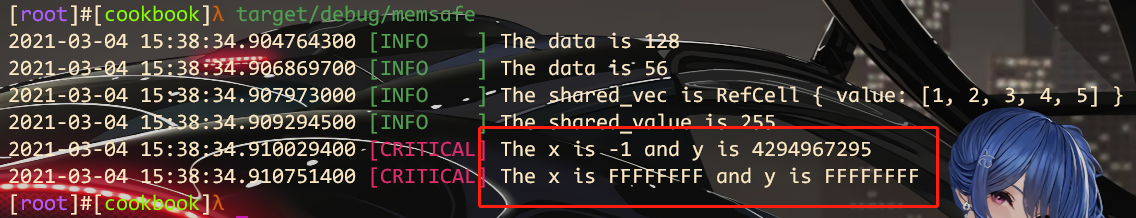
\includegraphics[width=\linewidth]{rust_raw_pointer.png}
  \caption{具有潜在错误的裸指针示例}
  \label{fig:rust_raw_pointer}
\end{figure}
x变成和y一样的值的原因在于:对指向y的指针类型做了转换,让它以为自己指向的是i64
类型,恰巧x就在y旁边,y被修改的同时,就顺带把x也修改了。因此,使用unsafe必须特别
小心。

在通常的情况下,虽然可以通过引用+mut的方式,可以阻止大部分的内存不安全问题,但是
由于引用+mut的强限制性,也为带来一些比较麻烦和无奈的问题,比如下面的代码:
\begin{code-block}{rust}
#[derive(Debug)]
struct Tuple {
    first: u8,
    second: u8,
    third: u8,
}
fn main() {
    let mut t = Tuple {
        first: 0,
        second: 1,
        third: 2,
    };
    let pa = &mut t.first;
    let pb = &mut t.second;
    let pc = &mut t.third;
    *pc += 10;
    info!("{:?}", t);
}
\end{code-block}
上述代码是正确无误的,可以正常编译和运行,但是,如果我们将结构体变成数组,问题就
出现了:
\begin{code-block}{rust}
fn main() {
    let mut array_x = [1_i32, 2, 8];
    let pa = &mut array_x[0];
    let pb = &mut array_x[1];
    *pb += 10;
    info!("{:?}", t);
}
\end{code-block}
上述代码在Rust 1.50.0版本之前就会出现错误:
\begin{code-block}{bash}
error: cannot borrow `x[..]` as mutable more than once at a time
\end{code-block}
原因在于,在Rust 1.50.0版本之前的结构体当中,pa,pb和pc指向不同的内存区域;
但是在数据当中,Rust编译器会将[\_]识别为一个整体,而\&[0], \&[1]之间都属于重叠,
将pa和pb判断为存在别名关系,即pa和pb实质上相同,违反了借用规则,因此无法通过编译。
采用引用分割才能进行解决:
\begin{code-block}{bash}
let mut array_x = [1_i32, 2, 3];
// 通过split_at_mut将数组切分成2个一定不会重叠的切片
let (first, rest): (&mut [i32], &mut [i32]) = array_x.split_at_mut(1);
let (second, third): (&mut [i32], &mut [i32]) = rest.split_at_mut(1);
first[0] += 100;
second[0] += 200;
third[0] += 300;
info!("{:?}", array_x);
\end{code-block}

由于Rust的目标是系统级的语言,必然需要具备操作硬件,以及裸设备的能力。而这些能力,
在C/C++的表述当中,通常是采用共用体(Union)实现的。为了与之兼容,Rust当中也引入了
Union数据结构,其主要的使用形式如下:
\begin{code-block}{rust}
#[repr(C)]
pub union U {
    pub i: u32,
    pub f: f32,
}

#[repr(C)]
pub struct Value {
    pub tag: u8,
    pub value: U,
}
\end{code-block}
其中,\#[repr(C)]必须使用,因为union的使用场景本身就是为了和C/C++进行对接,表示
该联合体使用和C/C++一样的内存布局。由于在字段当中使用了union,因此,结构体Value
也必须添加repr属性,否则会出现未定义的错误。而在使用的时候,则更加需要注意,只要
是涉及到读取联合体的字段,则必须使用unsafe:
\begin{code-block}{rust}
// 禁用illegal_floating_point_literal_pattern警告
#[allow(illegal_floating_point_literal_pattern)]
pub fn is_zero(v: &Value) -> bool {
    unsafe {
        match &v {
            Value {
                tag: Tag::I,
                value: U { i: 0 },
            } => true,
            Value {
                tag: Tag::F,
                // 会出现#[warn(illegal_floating_point_literal_pattern)]警告
                // 目前rust正在修复该问题
                value: U { f: 0.0 },
            } => true,
            _ => false,
        }
    }
}
\end{code-block}

Rust所有的unsafe实际都来源于性能和C的结合(比如写linux内核模块),因此原生指针
在unsafe当中最为常用。其主要的用途如下:
\begin{itemize}
  \item 在必要的时候跳过Rust安全检查:有的情况下,程序逻辑不会有任何内存安全的问题,原生指针可以跳过安全检查,提升性能
  \item 与C语言进行交互,必须使用原生指针
\end{itemize}

空指针在C语言当中非常常见,Rust当中也可以创建原生的空指针,也可以利用原生指针修改
数据:
\begin{code-block}{rust}
// 创建一个指向unsigned char的原生null指针
let pointer: *const u8 = std::ptr::null();
// 判断指针是否为空
assert!(pointer.is_null());

let mut s = [1, 2, 3];
// 创建一个可变的指针,该指针指向一个unsigned int的数组
let pointer: *mut u32 = s.as_mut_ptr();
assert!(!pointer.is_null());

unsafe {
    // 访问s[1]
    info!("The offset 1 is {}", *pointer.offset(1));
    // 访问s[2]
    info!("The offset 2 is {}", *pointer.offset(2));
    // 修改s[2]
    *pointer.offset(2) = 4;
    info!("The offset 2 is {}", *pointer.offset(2));
    // 将s[2]先转换成u8,然后再转换成char
    info!("The offset 2 is {}", *pointer.offset(2) as u8 as char);
}

info!("The final result of s is {:?}", s);
\end{code-block}

\section{杂项与技巧}

\subsection{预处理脚本与依赖关系}
在Rust当中,有的时候需要传递环境变量(编译期间)给源代码,生成特定的内容,此时
如果是直接在源代码当中进行环境变量的获取,则有可能获取到的是错误的信息。这种情况下
可以使用\colorblock{build.rs}脚本进行预处理。包含了该脚本的Rust工程结构大致如下:
\begin{figure}[H]
  \centering
  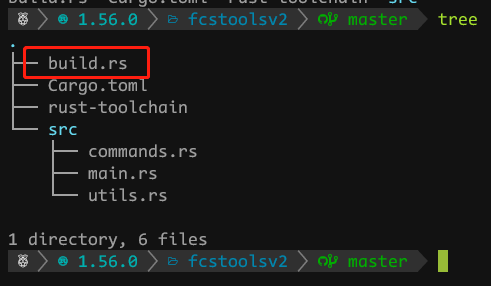
\includegraphics[width=\linewidth]{rust_build_rs.png}
  \caption{包含build.rs的工程结构}
  \label{fig:rust_build_rs}
\end{figure}

一个具体的build.rs实例如下:
\begin{code-block}{rust}
use std::process::Command;

fn main() {
    let output = Command::new("git")
        .args(&["rev-parse", "HEAD"])
        .output()
        .unwrap();
    let git_hash = String::from_utf8(output.stdout).unwrap();

    let __status__ = Command::new("git")
        .args(&["status", "--short"])
        .output()
        .unwrap();

    if "" != String::from_utf8(__status__.stdout).unwrap() {
        println!(
            "cargo:rustc-env=GIT_HASH={}-dirty",
            git_hash.trim_end_matches('\n')
        );
    } else {
        println!("cargo:rustc-env=GIT_HASH={}", git_hash);
    }
}
\end{code-block}

而在真正的源代码当中,使用则类似如下:
\begin{code-block}{rust}
...
let msg = format!(
    "For maintenance the AI Edge Platform, \nbuilt githash {}",
    env!("GIT_HASH"),
);
...
\end{code-block}

默认情况下,build.rs只会使用Rust标准库当中的所有函数和方法,即使是工程的Cargo.toml
文件的\codeinline{toml}{[dependencies]}引入了需要的依赖关系,build.rs仍然无法识别
相关的依赖包。如果需要在build.rs当中使用第三方的开发库,则需要修改工程的Cargo.toml
文件,添加如下的内容:
\begin{code-block}{toml}
# 表示给build.rs使用的依赖库
[build-dependencies]
chrono = "0.4.19"
\end{code-block}

注意,\codeinline{toml}{[dependencies]}和\codeinline{rust}{[build-dependencies]}当中
的依赖库是相互独立不影响的。如果build.rs当中的执行结果和预期的不一致,则可以直接
使用\codeinline{rust}{println!}进行输出打印,但是,这些信息不会在控制台上显示出来,
而是在\codeinline{bash}{target/xxx/build/yyy/output}当中,可以直接进行查看。

\subsection{性能优化与编码习惯}
Rust本身是一种高性能的编程语言,但是良好的编程习惯可以充分的发挥其高性能的特点,
一些习惯性的操作,也可以明显的提升代码的性能,性能优化是永恒的主题。最常见的优化
手段就是在编译代码的时候,使用\codeinline{bash}{--release}参数,release版的运行速度
通常比调试版快很多。

此外,链接时间优化(LTO)是一种整体的程序优化技术,通常可以将运行时性能提高10-20%
甚至更多,但代价是增加构建时间,不过这是值得的。启用LTO需要修改\codeinline{bash}{Cargo.toml},
具体改动如下:
\begin{code-block}{toml}
[profile.release]
lto = true
\end{code-block}

使用上述的配置参数,Rust会尝试对所有的crate进行优化(包括依赖关系),即所谓的“胖优化(fat)”。
如果不需要这么“激进”的优化策略,则可以设置\codeinline{toml}{lto = "thin"}。

从Rust1.60(2022-04-07)开始,Cargo的配置文件toml新增了一个项,专门用于对生成的二进制
文件进行文件缩小(strip)操作:
\begin{code-block}{toml}
[profile.release]
strip = true
\end{code-block}
如果是使用之前的版本,则该配置项等价于如下的命令:
\begin{code-block}{bash}
RUSTFLAGS='-C link-arg=-s' cargo build --release
\end{code-block}

如果需要去除生成的二进制文件当中的debug信息,默认情况下,不需要对配置文件做任何修改,
其等价于如下的命令:
\begin{code-block}{bash}
# 主要是-C debuginfo=0
RUSTFLAGS='-C link-arg=-s -C debuginfo=0' cargo build --release
\end{code-block}

如果需要在二进制文件当中包含debug信息,则可以将上述命令当中的debuginfo修改为其他
值,包括1和2。当然,也可以修改配置文件:
\begin{code-block}{toml}
[profile.release]
debug = true
\end{code-block}

在代码的编译过程当中,Rust编译器会将crate分割为多个代码生成单元(codegen units),
从而实现并行化编译,加快速度。但这个行为有可能会导致忽略一些潜在的优化。因此,如果
有必要,可以将分割的数目变少,以此来加大优化的程度:
\begin{code-block}{toml}
[profile.release]
codegen-units = 1
\end{code-block}
但codegen的数目如果比较小,会导致编译过程变长,也有一定的可能导致程序运行变慢。因此
该方式的使用需要进行综合权衡。

如果不需要考虑生成二进制文件的可移植性,则可以考虑充分利用当前运行环境的CPU特性,
自动选择最佳的CPU指令,从而极大程度上提升程序的性能:
\begin{code-block}{bash}
RUSTFLAGS="-C target-cpu=native" cargo build --release
\end{code-block}

更多的优化措施和策略,则需要靠开发人员自己进行实现。通常情况下,可以使用\codeinline{bash}{clippy}
工具,对代码进行分析,找出代码当中的不合理地方,然后加以修正:
\begin{code-block}{bash}
cargo clippy
\end{code-block}
该工具可以作为Rust代码风格的重要参考和指导,同样的,它也能针对代码编写的性能提出建议。

但是,rust的release以及优化选项可能会对程序的功能造成影响,比如,slog的debug/trace
级别的日志就会因为release的原因被优化,从而无法正常输出。遇到这种情况只能是具体
问题具体分析。比如slog的解决方法就是在Cargo.toml当中添加特殊的配置项:

\begin{code-block}{toml}
slog = {version = "2.7.0", features = ["max_level_trace", "release_max_level_trace"]}
\end{code-block}

\section{常见错误处理方法}
由于很多代码都是第三方的,而Rust本身也在不断的发展,有可能出现版本不兼容或者特性
不兼容的情况,此时,则需要进行相关的修改。比如下面的一种错误:
\begin{figure}[H]
  \centering
  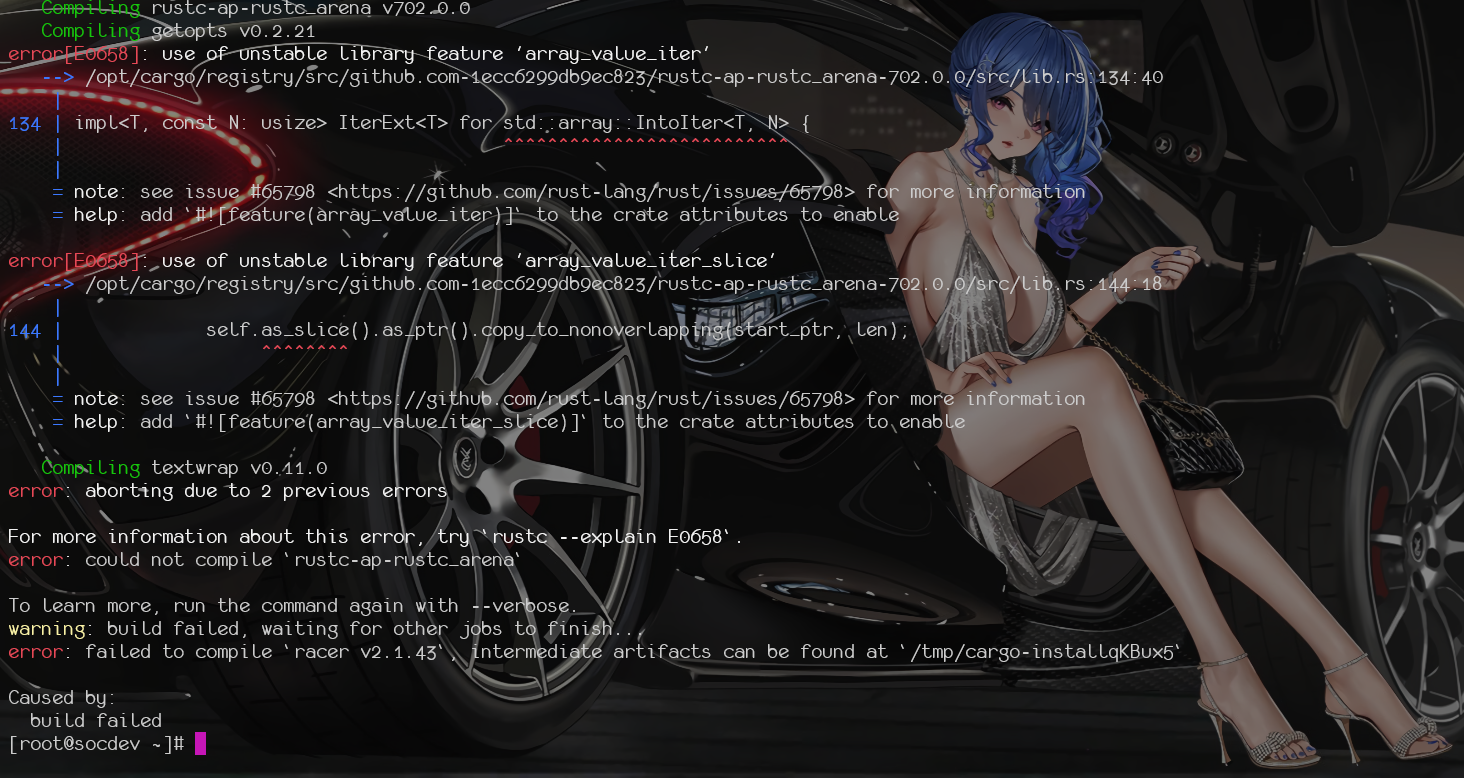
\includegraphics[width=\linewidth]{rust_feature_error.png}
  \caption{缺少特性支持编译失败}
  \label{fig:rust_feature_error}
\end{figure}
遇到这种错误,则需要直接修改对应的类库的源代码。以上述错误为例,编译的help表示
需要添加代码\codeinline{bash}{add `#![feature(array_value_iter_slice)]` to the crate attributes to enable},
则我们应当在对应的crate的lib.rs的头部当中,添加内容如下:
\begin{figure}[H]
  \centering
  
\includegraphics[width=\linewidth]{rust_feature_add.png}
  \caption{增加特性支持}
  \label{fig:rust_feature_add}
\end{figure}

\section{死灵书与实践}

\subsection{随机数实践}
Rust的随机数模块并不包含在标准库当中,需要使用rand这个crate,其基本的使用如下:
\begin{code-block}{rust}
use rand::distributions::{Distribution, Uniform};
use rand::seq::IteratorRandom;
use rand::Rng;
fn main() {
    let mut rng = rand::thread_rng();
    // 生成随机数
    info!("The float64 rand number is {}", rng.gen::<f64>());
    info!("The u32 rand number is {}", rng.gen::<u32>());
    info!("The i32 rand number is {}", rng.gen::<i32>());
    info!("The u8 rand number is {}", rng.gen::<u8>());
    // 从指定区间生成随机数
    info!("The range rand number is {}", rng.gen_range(0..100));
    info!(
        "The range rand float number is {}",
        rng.gen_range(10.0..50.0)
    );
    // 从[0, 5]生成随机数
    info!("The range rand number is {}", rng.gen_range(0..=5));
    // 定义[1, 7)的均匀分布
    let die = Uniform::from(1..7);
    // 从该分布当中生成采样
    let throw = die.sample(&mut rng);
    info!("The sample of uniform is {:>width$}", throw, width = 5);
    // 生成多个随机数
    let tuple: (u8, u8, u8) = rng.gen();
    info!("The tuple of random is {:?}", tuple);
    // 生成随机数组
    let array: [u8; 6] = rng.gen();
    info!("The array of random is {:?}", array);
    let mut exsit_array: [u8; 5] = [1, 2, 34, 5, 6];
    // 使用随机数填充已存在的数组
    rng.fill(&mut exsit_array);
    info!("The array of random is {:?}", exsit_array);
    // 从均匀分布当中随机采样3个数据
    // 得到的结果可能出现重复的情况
    let samples: Vec<u8> = (&mut rng).sample_iter(die).take(3).collect();
    info!("The samples of sample range 1..7 is {:?}", samples);
    let v = vec![1, 2, 3, 4, 5];
    // 从vec当中采样4个数据,得到的结果不会重复
    let sample = v.iter().choose_multiple(&mut rng, 4);
    info!("The samples of sample range 1..5 is {:?}", sample);
    let sample: Vec<u8> = (1..=10).choose_multiple(&mut rng, 4);
    info!("The samples of sample range 1..10 is {:?}", sample);
}
\end{code-block}

Rust的rand crate不仅可以生成随机数,也可以生成自定义的随机数据,比如:
\begin{code-block}{rust}
use rand::distributions::{Distribution, Standard, Uniform};
use rand::seq::IteratorRandom;
use rand::Rng;
struct Point {
    x: u8,
    y: u8,
}
impl fmt::Display for Point {
    fn fmt(&self, f: &mut fmt::Formatter) -> fmt::Result {
        write!(f, "x: {}, y: {}", self.x, self.y)
    }
}
// 在 Point 类型之上,对Standard实现Distribution trait,使得Point可以被gen函数随机生成
impl Distribution<Point> for Standard {
    // 默认的实现方法
    fn sample<R: Rng + ?Sized>(&self, rng: &mut R) -> Point {
        let (rand_x, rand_y) = rng.gen();
        Point {
            x: rand_x,
            y: rand_y,
        }
    }
}
fn main() {
    let mut rng = rand::thread_rng();
    let rand_point = rng.gen::<Point>();
    info!("The rand_point is {}", rand_point);
}
\end{code-block}

同样的,可以生成随机的字符串:
\begin{code-block}{rust}
use rand::distributions::{Alphanumeric, Distribution, Standard, Uniform};
use rand::seq::IteratorRandom;
use rand::Rng;
fn main() {
    let mut rng = rand::thread_rng();
    let rand_string: String = (&mut rng)
        // 从a-z,A-Z以及0-9当中进行选择
        .sample_iter(&Alphanumeric)
        // 获取其中的10个元素
        .take(10)
        // 默认的结果是char类型,需要继续转换成String
        .map(char::from)
        .collect();
    info!("The rand_string is {}", rand_string);
}
\end{code-block}

如果默认的字符集不满足要求,还可以自定义字符集,比如下面的示例:
\begin{code-block}{rust}
use rand::distributions::{Alphanumeric, Distribution, Standard, Uniform};
use rand::seq::IteratorRandom;
use rand::Rng;
const CHARSET: &[u8] = b"ABCDEFGHIJKLMNOPQRSTUVWXYZ\
    abcdefghijklmnopqrstuvwxyz\
    0123456789)(*&^%$#@!~";
const PASSWORD_LEN: usize = 10;
fn main() {
    let mut rng = rand::thread_rng();
    let password: String = (0..PASSWORD_LEN)
        .map(|_| {
            let idx = rng.gen_range(0..CHARSET.len());
            CHARSET[idx] as char
        })
        .collect();
    info!("The password is {}", password);
    // 也可以更换成之前的采样函数,看起来更为精炼
    let passwd: String = CHARSET
        .choose_multiple(&mut rng, 10)
        .map(|r| *r as char)
        .collect();
    info!("The password is {}", passwd);
}
\end{code-block}

同样的,针对自定义的数据类型,同样可以采用采样方法,进行随机数据的提取:
\begin{code-block}{rust}
use rand::distributions::{Alphanumeric, Distribution, Standard, Uniform};
use rand::seq::IteratorRandom;
use rand::Rng;
#[derive(Debug)]
struct Person {
    name: String,
    age: u8,
}
fn main() {
    let mut rng = rand::thread_rng();
    let persons = vec![
        Person {
            name: "lucifer".to_string(),
            age: 18,
        },
        Person {
            name: "titans".to_string(),
            age: 19,
        },
        Person {
            name: "garuda".to_string(),
            age: 36,
        },
    ];
    // 从person的vec当中,随机抽取2个元素
    let rand_person: Vec<_> = persons.choose_multiple(&mut rng, 2).collect();
    info!("The rand person is {:?}", rand_person);
}
\end{code-block}

\subsection{常见的设计模式}
建造者模式是Rust当中最常用的设计模式之一,其主旨思想在于将可变和不可变进行分离,
一种基本的示例如下:
\begin{code-block}{rust}
use std::f64::consts;
pub struct Circle {
    radius: f64,
}
pub struct CircleBuilder {
    radius: f64,
}
impl Circle {
    pub fn new() -> CircleBuilder {
        CircleBuilder { radius: 0.0 }
    }
    pub fn area(&self) -> f64 {
        self.radius * self.radius * consts::PI
    }
}
impl CircleBuilder {
    pub fn radius(&mut self, radius: f64) -> &mut CircleBuilder {
        self.radius = radius;
        self
    }
    pub fn build(&self) -> Circle {
        Circle {
            radius: self.radius,
        }
    }
}
\end{code-block}

\subsection{排序}
Rust的整数型数组和向量(Vector)的排序是相同的,可以使用相同的方式进行,即采用
sort以及sort\_unstable进行。其中,sort是稳定排序(即不重新排序相等的元素),
sort\_unstable是不稳定排序,\colorblock{但是通常情况下速度更快},并且不会进行辅助内存的分配。
\begin{code-block}{rust}
let mut v = vec![2, 21, 12, 32, 12, 45, 90];
v.sort_unstable();
info!("The sorted vector is {:?}", v);
let mut array = [2, 23, 12, 12, 98, 100, 21];
array.sort_unstable();
info!("The sorted array is {:?}", array);
\end{code-block}
默认情况下,排序操作使用的是升序,但是可以通过定制,修改排序方式:
\begin{code-block}{rust}
let mut v = vec![2, 21, 12, 32, 12, 45, 90];
// 降序排列,可替换成v.sort_by
v.sort_unstable_by(|a, b| b.cmp(a));
info!("The sorted vector is {:?}", v);
let mut array = [2i32, -23, 12, 12, 98, -100, 21];
// 根据绝对值升序排列,可以根据其他关键字进行排序
array.sort_unstable_by_key(|k| k.abs());
info!("The sorted array is {:?}", array);
// 根据字符顺序排列,带有缓存cache,闭包函数通常只执行一次,比无缓存的快速
let mut xx = [-5i32, 4, 32, -3, 2];
xx.sort_by_cached_key(|k| k.to_string());
// 字符串排序
let mut array = ["lucifer", "titans", "asura", "garuda"];
array.sort_unstable_by_key(|item| item.to_string());
info!("The string array is {:?}", array);
let mut array = [
    "lucifer".to_string(),
    "titans".to_string(),
    "asura".to_string(),
    "garuda".to_string(),
];
// 可以转换成切片
// array[..].sort_unstable_by_key(|item| item.to_string());
// info!("The string array is {:?}", array);
array.sort_unstable_by_key(|item| item.to_string());
info!("The string array is {:?}", array);
\end{code-block}

浮点数的排序和最值操作,参见\colorunderlineref{float_sort}

除了基础数据类型可以进行排序,同样可以针对复合数据类型进行排序。在针对复合数据
类型排序时,需要实现\colorblock{Eq,PartialEq,Ord和PartialOrd}这几个trait:
\begin{code-block}{rust}
#[derive(Eq, PartialEq, Ord, PartialOrd, Debug)]
struct Student {
    name: String,
    age: u8,
}
fn main() {
    let mut stu = [
        Student {
            name: "lucifer".to_string(),
            age: 18,
        },
        Student {
            name: "garuda".to_string(),
            age: 36,
        },
    ];
    // 按照自然序列(name)
    stu.sort();
    info!("The students is {:?}", stu);
    // 根据年龄
    stu.sort_unstable_by(|first, second| first.age.cmp(&second.age));
    info!("The students is {:?}", stu);
}
\end{code-block}

\subsection{压缩与解压}
Rust可以实现文件的压缩与解压,在Linux环境下,通常使用\href{https://github.com/alexcrichton/tar-rs}{tar}(归档)
和\href{https://github.com/rust-lang/flate2-rs}{flate2}(压缩解压),比如Linux下常见的tar.gz文件的处理:
\begin{code-block}{rust}
use flate2::read::GzDecoder;
use flate2::write::GzEncoder;
use flate2::Compression;
use tar::Archive;

let path = "/root/py3.tar.gz";
let targz = match File::open(path) {
    Ok(file) => file,
    Err(error) => {
        crit!("Failed to open the file {}: {}", path, error.to_string());
    }
};
// gz文件的解码器
let tar = GzDecoder::new(targz);
// tar的管理器
let mut archive = Archive::new(tar);
// 将tar.gz解压
match archive.unpack(".") {
    Ok(_) => info!("Sucess to unpack the tar.gz file"),
    Err(error) => {
        crit!("Failed to unpark the tar.gz file: {:?}", error);
    }
}
// 创建tar.gz文件
let targz = match File::create("log.tar.gz") {
    Ok(file) => file,
    Err(error) => {
        crit!(
            "Failed to create the log.tar.gz file : {}",
            error.to_string()
        );
    }
};
// 创建gz文件的编码器,压缩算法使用默认
let encoder = GzEncoder::new(targz, Compression::default());
let mut tarfile = tar::Builder::new(encoder);
// 将文件添加到tar.gz文件当中
match tarfile.append_dir_all("log", "/var/log") {
    Ok(_) => info!("log.tar.gz created sucessful"),
    Err(error) => {
        fs::remove_file("log.tar.gz").unwrap_or_else(|why| {
            error!("Cannot remove the log.tar.gz: {:?}", why.to_string())
        });
        crit!("Failed to park the tar.gz file: {:?}", error);
    }
}
\end{code-block}

当然,归档和压缩也可以单独使用:
\begin{code-block}{rust}
use flate2::read::GzDecoder;
use flate2::write::GzEncoder;
use flate2::Compression;
use tar::Archive;
let tarf = match File::create("log.tar") {
    Ok(file) => file,
    Err(error) => {
        crit!("Failed to create the log.tar file : {}", error.to_string());
    }
};
// 注意和gz文件不一样,只是归档,则不需要创建编码器
let mut tar_file = tar::Builder::new(tarf);
match tar_file.append_dir_all("log", "/var/log") {
    Ok(_) => info!("log.tar created sucessful"),
    Err(error) => {
        fs::remove_file("log.tar")
            .unwrap_or_else(|why| error!("Cannot remove the log.tar: {:?}", why.to_string()));
        crit!("Failed to park the tar.gz file: {:?}", error);
    }
}
let path = "/root/log.tar";
let tarball = match File::open(path) {
    Ok(file) => file,
    Err(error) => {
        crit!("Failed to open the file {}: {}", path, error.to_string());
    }
};
// 同样的,解压tar文件,不需要创建解码器
let mut archive = Archive::new(tarball);
match archive.unpack(".") {
    Ok(_) => info!("Sucess to unpack the tar file"),
    Err(error) => {
        crit!("Failed to unpark the tar file: {:?}", error);
    }
}
\end{code-block}
